\documentclass[crop,border={2pt 0 2pt 0},tikz]{standalone}
\usepackage{tikz-3dplot}
\usetikzlibrary{decorations.markings, backgrounds, calc, arrows.meta, bending}
\tikzset{>=latex}
\tikzset{->-/.style={decoration={
    markings,
    mark=at position .5 with {\arrow{>}} },postaction={decorate}}
}

\tikzset{-./.style={decoration={
    markings,
    mark=at position 0.999 with {\pgfuseplotmark{*}} },postaction={decorate}}
}

\tikzset{->-./.style={decoration={
    markings,
    mark=at position 0.6 with {\arrow{>}},
    mark=at position 1 with {\pgfuseplotmark{*}}
    },postaction={decorate}}
}

\tikzset{->->-./.style={decoration={
    markings,
    mark=at position 0.3 with {\arrow{>[bend]}},
    mark=at position 0.8 with {\arrow{>[bend]}},
    mark=at position 0.999 with {\pgfuseplotmark{*}}
    },postaction={decorate}}
}

\tikzset{-<-./.style={decoration={
    markings,
    mark=at position 0.6 with {\arrow{<}},
    mark=at position 1 with {\pgfuseplotmark{*}}
    },postaction={decorate}}
}
\begin{document}
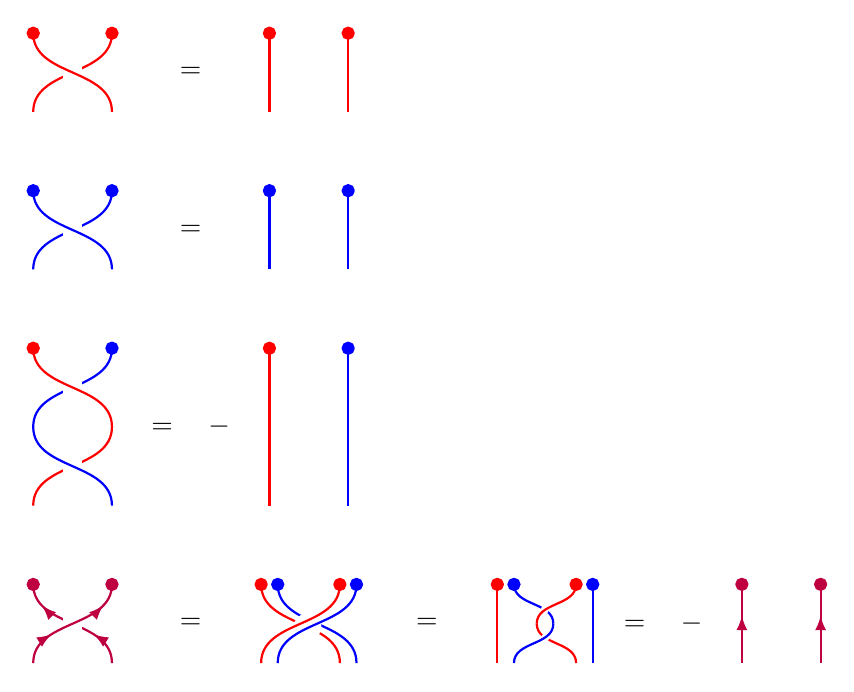
\begin{tikzpicture}[line join = round]

\draw[-.,red, thick] (0,0) to [out=90, in=270] node[pos = 0.5, fill=white, anchor=center]{} +(1,1);
\draw[-.,red, thick](1,0) to [out=90, in=270] +(-1,1);
\node[anchor=center] at (2, 0.5) {$=$};
\draw[-.,red, thick] (3,0) -- +(0,1);
\draw[-.,red, thick](4,0) -- +(0,1);

\begin{scope}[yshift = -2cm]
    \draw[-.,blue, thick] (0,0) to [out=90, in=270] node[pos = 0.5, fill=white, anchor=center]{} +(1,1);
    \draw[-.,blue, thick](1,0) to [out=90, in=270] +(-1,1);
    \node[anchor=center] at (2, 0.5) {$=$};
    \draw[-.,blue, thick] (3,0) -- +(0,1);
    \draw[-.,blue, thick](4,0) -- +(0,1);
\end{scope}

\begin{scope}[yshift = -5cm]
    \draw[red, thick] (0,0) to [out=90, in=270] node[pos = 0.5, fill=white, anchor=center]{} (1,1) ;

    \draw[blue, thick](1,0) to [out=90, in=270] +(-1,1);
    \draw[-.,blue, thick](0,1) to [out=90, in=270] node[pos = 0.5, fill=white, anchor=center]{} +(1,1);

    \draw[-.,red, thick] (1,1) to [out=90, in=270] +(-1,1);
    
    \node[anchor=center] at (2, 1) {$= \ \ \ -$};

    \draw[-.,red, thick] (3,0) -- +(0,2);
    \draw[-.,blue, thick](4,0) -- +(0,2);
\end{scope}

\begin{scope}[yshift = -7cm]
    \draw[->->-.,purple, thick](1,0) to [out=90, in=270] node[pos = 0.5, fill=white, anchor=center]{} +(-1,1);
    \draw[->->-.,purple, thick] (0,0) to [out=90, in=270] +(1,1);
    
    \node[anchor=center] at (2, 0.5) {$=$};

    \draw[-.,blue, thick, xshift = 3](4,0) to [out=90, in=270] node[pos = 0.575, fill=white, anchor=center, circle,inner sep =0pt ,  minimum size= 3pt] {} +(-1,1);

    \draw[-.,red, thick, xshift = -3](4,0) to [out=90, in=270] node[pos = 0.44, fill=white, anchor=center, circle,inner sep =0pt ,  minimum size= 10pt]  {} +(-1,1);

    \draw[-.,red, thick, xshift = -3] (3,0) to [out=90, in=270] +(1,1);

    \draw[-.,blue, thick, xshift = 3] (3,0) to [out=90, in=270]  +(1,1);
   

    \node[anchor=center] at (5, 0.5) {$=$};

    \draw[-.,red, thick, xshift = -3] (6,0) -- +(0,1);

    \draw[-.,blue, thick, xshift = 3] (7,0) --  +(0,1);

    \draw[red, thick, xshift = -3] (7,0) to [out=90, in=270] node[pos = 0.7, fill=white, anchor=center, circle,inner sep =0pt ,  minimum size= 3pt]  {} +(-0.5,0.5) ;

    \draw[blue, thick, xshift = 3](6,0) to [out=90, in=270] +(0.5,0.5);
    \draw[-.,blue, thick, xshift = 3](6.5,0.5) to [out=90, in=270] node[pos = 0.3, fill=white, anchor=center, circle,inner sep =0pt ,  minimum size= 3pt]  {} +(-0.5,0.5);

    \draw[-.,red, thick, xshift = -3] (6.5,0.5) to [out=90, in=270] +(0.5,0.5);

    \node[anchor=center] at (8, 0.5) {$= \ \ \ -$};

    \draw[->-.,purple, thick] (9,0) -- +(0,1);
    \draw[->-.,purple, thick](10,0) -- +(0,1);


\end{scope}

% \draw[-.,red, thick] (0.1,-1.8) -- +(0,1);
% \draw[-.,blue, thick](0.3,-1.8) -- +(0,1);
% \node[anchor=center] at (0.6, -1.3) {$=$};
% \draw[->-.,purple, thick](1.0,-1.8) -- +(0,1) node[anchor=south, black] (psi) {$\psi$};

% \draw[-.,blue, thick] (0.1,-3.6) -- +(0,1);
% \draw[-.,red, thick](0.3,-3.6) -- +(0,1);
% \node[anchor=center] at (0.6, -3.1) {$=$};
% \draw[-<-.,purple, thick](1.0,-3.6) -- +(0,1);

\end{tikzpicture}

\end{document} 
